%Stima degli errori delle grandezze misurate (giustificare il metodo scelto)
%Valore finale della grandezza da determinare ed incertezza
%Ricordarsi di dare i valori con i rispettive errori e attenzione alle cifre significative!

%Sample: Table
%\begin{table}[!htbp]
%    {\par\centering
%    \begin{tabular}{ccccc}
%        \hline
%        Misura & $M \text{ (g)}$ & $\sigma_{M} \text{ (g)}$ & $L \text{ (cm)}$ & $\sigma_{L} \text{ (cm)}$ \\
%        \hline
%        1   &   324.2&   0.1 &   79.5    &   0.1\\
%        2   &   333.7&   0.1 &   79.6    &   0.1\\
%        3   &   344.1&   0.1 &   79.7    &   0.1\\
%        4   &   363.7&   0.1 &   80.0    &   0.1\\
%        5   &   383.4&   0.1 &   80.1    &   0.1\\
%        \hline
%    \end{tabular}
%    \par}
%    \caption{Lunghezza della corda in funzione delle masse appese}
%\end{table}


%Sample: Multiline values
%\begin{align*}
%    &M_{tot} = (20.6 \pm 0.1) \ \text{g} \\
%    &m_{g} = (3.2 \pm 0.1) \ \text{g} \\
%    &L_{r,tot} (77.5 \pm 0.1) \ \text{cm} \\
%    &L_{r} = (75.8 \pm 0.1) \ \text{cm} \\
%\end{align*}

%Sample: Single line value
%\[
%    L_{0}=(78.8 \pm 0.1) \ \text{cm}
%\]


%Sample: Chart
%\begin{center}
%\begin{tikzpicture}
%    \begin{axis}[
%        title=Determinazione costante elastica,
%        xlabel=$L \text{ (m)}$,
%        ylabel=$M_{s} \text{ (kg)}$,
%        minor y tick num=1,
%        minor x tick num=1,
%        x tick label style={
%            /pgf/number format/.cd,
%            fixed,
%            fixed zerofill,
%            precision=3,
%            /tikz/.cd
%        }
%    ]
%        \addplot[color=blue, domain=0.794:0.802]{x*9.079-6.893};
%        \addplot+[scatter, only marks, mark=o, error bars/.cd, y dir=both,y explicit, x dir=both, x explicit, error %mark=-]
%            coordinates {
%                (0.7950,0.3242)   +-  (0.001,0.0001)
%                (0.7960,0.3337)   +-  (0.001,0.0001)
%                (0.7970,0.3441)  +-  (0.001,0.0001)
%                (0.8000,0.3637)  +-  (0.001,0.0001)
%                (0.8010,0.3834)  +-  (0.001,0.0001)
%        };
%    \end{axis}
%\end{tikzpicture}
%\end{center}

\numberwithin{equation}{section}
\numberwithin{table}{section}
\numberwithin{figure}{section}
\subsection{Charge to mass ratio of the electron}
%The coil magnetic field is generated at its centre, as such, 
%We found the radius of the coil as the sum of the distance between their outer parts $d_{\text{ext}}$ , and their inner distance $d_{\text{int}}$ all divided by 2. We took three measures and use their arithmetic mean as the final value
%and use their arithmetic mean as the final value $x_f=(15.536\pm 0.015)$ cm. Their values, in centimetres, are shown below:
%\begin{table}[h!]
%    \centering
%        \begin{tabular}{|c|c|c|}
%            \hline
%            \textbf{$X_o$} & \textbf{$X_i$} & \textbf{$X_r$} \\
%            \hline
%            17.740 & 13.260 & 15.500 \\
%            \hline
%            17.786 & 13.342 & 15.564 \\
%            \hline
%            17.780 & 13.310 & 15.545 \\
%            \hline
%        \end{tabular} 
%\end{table}
%where $x_r$ is the radius of the coil.  
The measure of the distance between the two Helmholtz coils is done with a slide gauge, by taken 
the internal distance $d_{\text{int}}$ and external distance $d_{\text{ext}}$ between the coils.
The distance between the two coils in each set of measure $d$ is calculated as the semi sum of the distances. 

The following table represent the measures $d_{\text{int}}$, $d_{\text{ext}}$, and the calculate $d$:
\begin{table}[!htbp]
    {\par\centering
    \begin{tabular}{cccc}
        \hline
        Measure & $d_{\text{int}} \text{ (cm)}$ & $d_{\text{ext}} \text{ (cm)}$ & $d \text{ (cm)}$\\
        \hline
        1   &   13.260& 17.740&   15.500\\
        2   &   13.342& 17.786&   15.564\\
        3   &   13.310& 17.780&   15.545\\
        \hline
    \end{tabular}
    \par}
    \caption{External and internal distance between Helmholtz coils}
\end{table}

Given the three set of measures the distance between the coils $\bar{d}$, is calculated as the arithmetic mean of each  calculated distance, while the error $\sigma_{\bar{d}}$ is calculated as the standard error of the mean.
\begin{equation*}
    \sigma_{\bar{d}}=\frac{\sigma_d}{\sqrt{N}}
\end{equation*}
where $\sigma_d$ is the standard deviation and $N$ the number of measures.

Since the configuration of the equipment is such that the distance between the Helmholtz coils is equal to the radius of the coils $R_b$:
\[
    R_b=15.536 \pm 0.268 \ \text{cm}
\]


%We took the resolution of the nonius ($\pm 0.002$ cm) as the uncertainty on our measures; the one on the mean was $calculated as the standard error of the mean:
%\begin{equation*}
%    \sigma_{x_f}=\frac{\sigma}{\sqrt{n}}
%\end{equation*}
%where $\sigma$ is the standard deviation and n the number of measures.

Voltage $\Delta V$ and current intensity $I$ are measured with digital multimeters respectively with resolution of $\pm 0.1 \text{ V}$ and $\pm 0.001 \text{ A}$.
The diameter of the deflected beam of electrons is measured using a slide gauge with a resolution of $\pm 0.002 \text{ cm}$.
For each set we took two measures $D_1$ and $D_2$ as the distance between a pair a sliders which represent the diameter of the circle, and calculated the radius of the circle $R$ as the semi sum divided by two and the error of the radius $\sigma_R$ as the semi difference divided by two.

The following table shows the measure and electrons beam radius in orthogonal configuration:
\begin{table}[!htbp]
    {\par\centering
    \begin{tabular}{ccccccc}
        \hline
        Measure & $I \text{ (A)}$ & $\Delta V \text{ (V)}$ & $D_1 \text{ (cm)}$ & $D_2 \text{ (cm)}$ & $R \text{ (cm)}$ & $\sigma_R \text{ (cm)}$ \\
       \hline
       1   &   1.133&   162.5&   9.374&   9.190& 4.641 & 0.046\\
       2   &   1.187&   176.8&   9.120&   9.200& 4.580 & 0.020\\
       3   &   1.160&   195.5&  10.170&  10.100& 5.068 & 0.017\\
       4   &   1.375&   213.8&   9.044&   9.048& 4.523 & 0.001\\
       5   &   1.307&   224.5&   9.780&   9.778& 4.890 & 0.001\\
       6   &   1.554&   242.2&   8.550&   8.580& 4.283 & 0.007\\
       7   &   1.522&   257.8&   9.072&   9.040& 4.528 & 0.008\\
       8   &   1.607&   274.8&   8.980&   9.010& 4.498 & 0.007\\
       9   &   1.740&   295.9&   8.520&   8.522& 4.261 & 0.001\\
       10  &   1.240&   200.0&   9.550&   9.560& 4.778 & 0.003\\
       \hline
   \end{tabular}
   \par}
   \caption{Orthogonal configuration - Radius of the electron beam}
\end{table}

The following table shows the measure and electrons beam radius in parallel configuration:

\begin{table}[!htbp]
    {\par\centering
    \begin{tabular}{ccccccc}
        \hline
        Measure & $I \text{ (A)}$ & $\Delta V \text{ (V)}$ & $D_1 \text{ (cm)}$ & $D_2 \text{ (cm)}$ & $R \text{ (cm)}$ & $\sigma_R \text{ (cm)}$ \\
        \hline
        1   &   1.133&   149.2&   8.510&   8.450& 4.240&  0.015\\
        2   &   1.367&   166.7&   7.790&   7.770& 3.890&  0.005\\
        3   &   1.293&   179.4&   8.680&   8.650& 4.333&  0.008\\
        4   &   1.428&   193.1&   8.290&   8.320& 4.153&  0.008\\
        5   &   1.532&   209.0&   7.940&   7.944& 3.971&  0.010\\
        6   &   1.552&   226.1&   8.360&   8.362& 4.181&  0.001\\
        7   &   1.657&   240.8&   8.010&   8.000& 4.003&  0.003\\
        8   &   1.353&   257.7&  10.292&  10.260& 5.138&  0.008\\
        9   &   1.328&   272.6&  10.790&  10.800& 5.398&  0.003\\
        10  &   1.372&   292.2&  10.608&  10.620& 5.307&  0.003\\
        \hline
    \end{tabular}
    \par}
    \caption{Parallel configuration - Radius of the electron beam}
\end{table}

The following table shows the measure and electrons beam radius in antiparallel configuration:

\begin{table}[!htbp]
    {\par\centering
    \begin{tabular}{ccccccc}
        \hline
        Measure & $I \text{ (A)}$ & $\Delta V \text{ (V)}$ & $D_1 \text{ (cm)}$ & $D_2 \text{ (cm)}$ & $R \text{ (cm)}$ & $\sigma_R \text{ (cm)}$ \\
        \hline
        1   &   0.811&   151.6&  11.280&  11.300& 5.645&  0.005\\
        2   &   0.881&   181.2&  12.290&  12.400& 6.173&  0.028\\
        3   &   1.038&   212.6&  11.650&  11.620& 5.818&  0.008\\
        4   &   1.151&   242.6&  10.280&  10.190& 5.118&  0.023\\
        5   &   1.289&   272.7&  10.480&  10.470& 5.238&  0.003\\
        6   &   1.302&   296.9&  11.130&  11.111& 5.560&  0.005\\
        7   &   1.204&   259.4&  11.350&  11.200& 5.638&  0.038\\
        8   &   1.136&   228.2&  10.980&  10.990& 5.493&  0.003\\
        \hline
    \end{tabular}
    \par}
    \caption{Antiparallel configuration - Radius of the electron beam}
\end{table}

The coil's magnetic field can be calculated using:
\begin{equation*}
    B_z=\mu_0\frac{8}{5\sqrt{5}}\frac{NI}{R_b}
\end{equation*}
where $\mu_0$ is the vacuum magnetic permeability, N is the number of turns, I is the current intensity and $R_b$ is the coil radius. The uncertainty can be obtained through error propagation as:
\begin{equation*}
    \sigma_{B_z}=B_z \sqrt{\left(\frac{\sigma_I}{I}\right)^2+\left(\frac{\sigma_{R_b}}{R_b}\right)^2}
\end{equation*}
With the magnetic field we can ultimately find the e/m ratio as:
\begin{equation*}
    \frac{e}{m}=\frac{2\Delta V}{(B_zR)^2}
\end{equation*}
and used the linear regression formulas:
\begin{align*}
S_w &= \sum_{n=1}^N \frac{1}{\sigma_n^2} & \quad S_x &= \sum_{n=1}^N \frac{x_n}{\sigma_n^2} & \quad S_{xx} &= \sum_{n=1}^N \frac{x_n^2}{\sigma_n^2} \\
S_y &= \sum_{n=1}^N \frac{y_n}{\sigma_n^2} & \quad S_{xy} &= \sum_{n=1}^N \frac{x_n y_n}{\sigma_n^2}  & \quad \Delta &= S_{xx} S_w - S_x^2 \\
a &= \frac{S_{xy} S_w - S_x S_y}{\Delta} & \quad b &= \frac{S_x S_y - S_{xy} S_w}{\Delta} \\
\sigma_a &= \sqrt{\frac{S_w}{\Delta}} & \quad \sigma_b &= \sqrt{\frac{S_{xx}}{\Delta}} 
\end{align*}
where  $\sigma_n$ is the uncertainty on $(B_zR)^2$, $x_n$ is $2 \Delta V$ and  $y_n$ is $(B_zR)^2$, $a$ is the ratio $\frac{m}{e}$ and b is the intercept on axis $y$.
\begin{figure}[H]
    \centering
    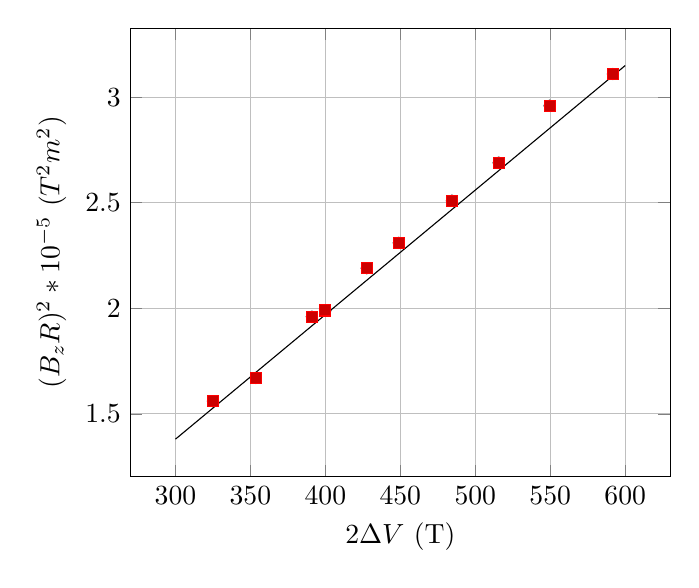
\begin{tikzpicture}
        \begin{axis}
        [
            xlabel={$2\Delta V$ (T)},
            ylabel={$(B_zR)^2*10^{-5}$ ($T^2m^2$)},
            grid=both,
            scatter/classes={
                a={mark=o,draw=black},
                b={mark=o,draw=black,fill=black}
            }
        ]
        \addplot[scatter,only marks,scatter src=explicit symbolic] 
            table[meta=label] {
              x     y    xerror yerror    label
            325     1.56   0.1     0.022      b
            353.6	1.67   0.1     0.014      a
            391	    1.96   0.1     0.014      a
            427.6	2.19   0.1     0.014      a
            449     2.31   0.1     0.014      a
            484.4   2.51   0.1       0        a
            515.6   2.69   0.1       0        a  
            549.6   2.96   0.1       0        a
            591.8   3.11   0.1       0        a
            400     1.99   0.1       0        a
         
        };
        \addplot+[
            only marks,
            error bars/.cd,
            x dir=both, x explicit,
            y dir=both, y explicit
        ] table[x=x, y=y, x error=xerror, y error=yerror] {
                x     y    xerror yerror    label
            325     1.56   0.1     0.022      b
            353.6	1.67   0.1     0.014      a
            391	    1.96   0.1     0.014      a
            427.6	2.19   0.1     0.014      a
            449     2.31   0.1     0.014      a
            484.4   2.51   0.1       0        a
            515.6   2.69   0.1       0        a  
            549.6   2.96   0.1       0        a
            591.8   3.11   0.1       0        a
            400     1.99   0.1       0        a
        };
        \addplot[
    domain=300:600,
    samples=100,
    color=black
] {0.0059*x - 0.39};
    \end{axis}
    \end{tikzpicture}
    \caption{Linear regression between $(B_zR)^2$ and the voltage for the orthogonal setup. }
\end{figure}

%paralello
\begin{figure}[H]
    \centering
    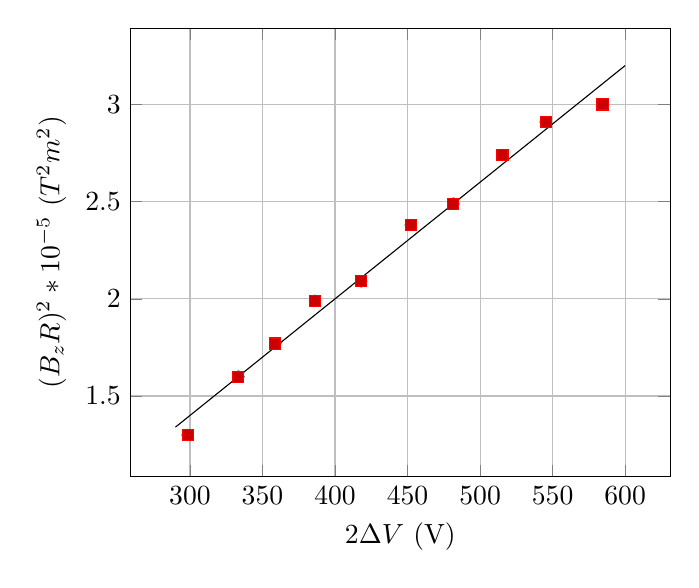
\begin{tikzpicture}
        \begin{axis}
        [
            xlabel={$2\Delta V$ (V)},
            ylabel={$(B_zR)^2*10^{-5}$ ($T^2m^2$)},
            grid=both,
            scatter/classes={
                a={mark=o,draw=black},
                b={mark=o,draw=black,fill=black}
            }
        ]
        \addplot[scatter,only marks,scatter src=explicit symbolic] 
            table[meta=label] {
              x     y    xerror yerror    label
            298.4   1.30   0.1     0.022      b
            333.4	1.60   0.1     0.014      a
            358.8   1.77   0.1     0.014      a
            386.2	1.99   0.1     0.014      a
            418     2.09   0.1     0.014      a
            452.2   2.38   0.1       0        a
            481.6   2.49   0.1       0        a  
            515.4   2.74   0.1       0        a
            545.2   2.91   0.1       0        a
            584.4   3.00   0.1       0        a
         
        };
        \addplot+[
            only marks,
            error bars/.cd,
            x dir=both, x explicit,
            y dir=both, y explicit
        ] table[x=x, y=y, x error=xerror, y error=yerror] {
             x     y    xerror yerror    label
            298.4   1.30   0.1     0.022      b
            333.4	1.60   0.1     0.014      a
            358.8   1.77   0.1     0.014      a
            386.2	1.99   0.1     0.014      a
            418     2.09   0.1     0.014      a
            452.2   2.38   0.1       0        a
            481.6   2.49   0.1       0        a  
            515.4   2.74   0.1       0        a
            545.2   2.91   0.1       0        a
            584.4   3.00   0.1       0        a
        };
        \addplot[
    domain=290:600,
    samples=100,
    color=black
] {0.0060*x - 0.40};
    \end{axis}
    \end{tikzpicture}
    \caption{Linear regression between $(B_zR)^2$ and the voltage for the parallel setup. }
\end{figure}

%antiparallelo

\begin{figure}[H]
    \centering
    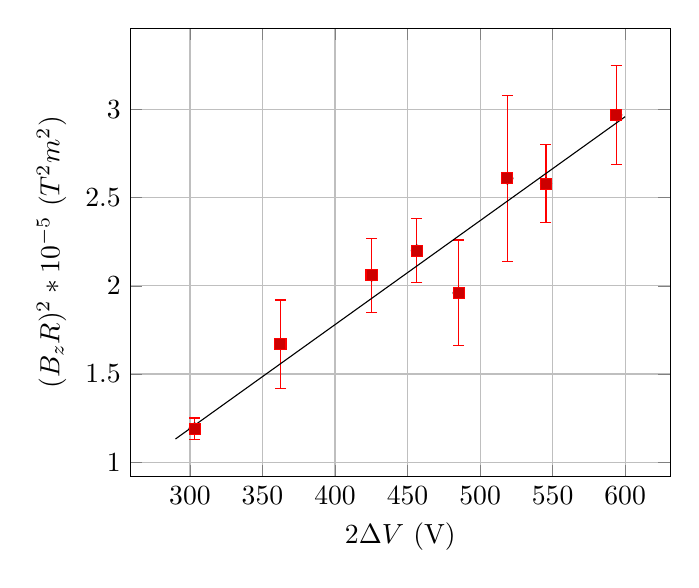
\begin{tikzpicture}
        \begin{axis}
        [
            xlabel={$2\Delta V$ (V)},
            ylabel={$(B_zR)^2*10^{-5}$ ($T^2m^2$)},
            grid=both,
            scatter/classes={
                a={mark=o,draw=black},
                b={mark=o,draw=black,fill=black}
            }
        ]
        \addplot[scatter,only marks,scatter src=explicit symbolic] 
            table[meta=label] {
              x     y    xerror yerror    label
            303.2   1.19   0.1     0.022      b
            362.4	1.67   0.1     0.014      a
            425.2   2.06   0.1     0.014      a
            485.2	1.96   0.1     0.014      a
            545.4   2.58   0.1     0.014      a
            593.8   2.97   0.1       0        a
            518.8   2.61   0.1       0        a  
            456.4   2.20   0.1       0        a
        };
        \addplot+[
            only marks,
            error bars/.cd,
            x dir=both, x explicit,
            y dir=both, y explicit
        ] table[x=x, y=y, x error=xerror, y error=yerror] {
               x     y    xerror yerror    label
            303.2   1.19   0.1     0.06      b
            362.4	1.67   0.1     0.25      a
            425.2   2.06   0.1     0.21      a
            485.2	1.96   0.1     0.30      a
            545.4   2.58   0.1     0.22      a
            593.8   2.97   0.1     0.28      a
            518.8   2.61   0.1     0.47      a  
            456.4   2.20   0.1     0.18      a
        };
        \addplot[
    domain=290:600,
    samples=100,
    color=black
] {0.0059*x - 0.58};
    \end{axis}
    \end{tikzpicture}
    \caption{Linear regression between $(B_zR)^2$ and the voltage for the antiparallel setup.}
\end{figure}
Note that the measure for the antiparallel setup have an higher error compared to others, this has led to a higher uncertainty on respective the e/m value.
The reduced chi squared $\chi_{red}^2$ for each configuration are:
\begin{align*}
    &\chi_{red}^2=10.5\,\,(Orthogonal)\\
    &\chi_{red}^2=55.7\,\,(Parallel)\\
    &\chi_{red}^2=0.32\,\,(Antiparallel)
\end{align*}
the reduced chi squared for the orthogonal and parallel setup shows an incompatibilty of the model with the measures. As we discussed later in the conclusion we thinks that this problem could relate with a wrong setup during the measures.
The final values were found to be:
\begin{align*}
    &\frac{e}{m}=(1.69\pm0.01)\, \mathrm{C/kg}\,\, \text{(Orthogonal)}\\
    &\frac{e}{m}=(1.66\pm0.01)\, \mathrm{C/kg}\,\, \text{(Parallel)}\\
    &\frac{e}{m}=(1.67\pm0.16)\, \mathrm{C/kg}\,\, \text{(Antiparallel)}\\
\end{align*}
which does not correlate but antiparallel, with the accepted value of:
\begin{equation*}
    \frac{e}{m}=1.76\,\,\, \mathrm{C/kg}
\end{equation*}



\subsection{Horizontal component's intensity of Earth's magnetic field}
For each fixed angle $\theta$ we measured the intensity $I$ two times (clockwise $I_c$ and counter-clockwise $I_{cc}$) and took their mean as the final value:
\begin{table}[!htbp]
    {\par\centering
    \begin{tabular}{cccc}
        \hline
        $I_c \text{ (mA)}$ & $I_{cc} \text{ (mA)}$ &  $\bar{I} \text{ (mA)}$ & $\theta$ \\
        \hline
        14.33 & 15.76 & 15.05 & $45^{\circ}$  \\
        17.30 & 20.20 & 18.75 & $50^{\circ}$  \\
        21.38 & 22.60 & 21.99 & $55^{\circ}$  \\
        26.55 & 26.29 & 26.42 & $60^{\circ}$  \\
        34.98 & 33.65 & 34.32 & $65^{\circ}$  \\
        \hline
    \end{tabular}
    \par}
    \caption{Earth's magnetic field - Measure of needle deflection clokwise and counter clockwise}
\end{table}

The uncertainty on the intensity is the last digit provide by the device ($\pm 0.01 \text{mA}$) while the one on the angle is the protractor's resolution ($\pm 1^{\circ}$).
The coil magnetic field's components $B_z$ and $B_r$ are provided for fixed $\theta$ and needle lenght $R$:
\begin{table}[!htbp]
    {\par\centering
    \begin{tabular}{cc}
        \hline
        $B_z$ (mT) & $B_r$ (mT) \\
        \hline
        0.15438 & 0.00228 \\
        0.15471 & 0.00167 \\
        0.15480 & 0.00110 \\
        0.15472 & 0.00062 \\
        0.15450 & 0.00025 \\
        \hline
    \end{tabular}
    \par}
    \caption{Tabulated values for the orthogonal ($B_z$) and parallel ($B_r$) coil magnetic field's components.}
\end{table}

We can now calculate the Horizontal component of Earth's magnetic fiels ($B_t$) as:
\begin{equation*}
    B_t=\frac{I}{I_0}(B_z \cot{(\theta)}+B_r)
\end{equation*}
where $I_0=(100\pm 1)$ mA is the intensity of the coil current power source, and calculated its uncertainty:
\begin{align*}
    &\sigma_{B_t}^2 = \left( \frac{1}{I_0} \left( B_z \cot(\theta) + B_r \right) \sigma_I \right)^2 + \left( -\frac{I}{I_0^2} \left( B_z \cot(\theta) + B_r \right) \sigma_{I_0} \right)^2 + \left( \frac{I}{I_0} \cot(\theta) \sigma_{B_z} \right)^2 \\
    &+ \left( \frac{I}{I_0} B_z \left( -\csc^2(\theta) \right) \sigma_\theta \right)^2 + \left( \frac{I}{I_0} \sigma_{B_r} \right)^2
\end{align*}
Its values for each measurement are shown below:
\begin{table}[!htbp]
    {\par\centering
    \begin{tabular}{cc}
        \hline
        $B_t$ ($\mu$T) & $\sigma_{B_t}$ ($\mu$T) \\
        \hline
        23.57 & 1.40 \\
        24.65 & 2.11 \\
        24.08 & 1.13 \\
        23.76 & 0.99 \\
        24.81 & 1.25 \\
        \hline
    \end{tabular}
    \par}
    \caption{Calculated value of $B_t$ for each deflection}
\end{table}

We lastly calculated the final value as the weighted arithmetic mean of these values finding:
\begin{equation*}
    B_{tf}=(24.08\pm0.56)\,\, \mu\mathrm{T}
\end{equation*}

